\documentclass{AIAA}
\usepackage{amsmath}
\usepackage{amssymb}
\usepackage{graphicx}
\usepackage{verbatim}
%\usepackage{hyperref}
%\usepackage{authblk}
%\usepackage{setspace}




\begin{document}
\title{Improvements to the Ion Doppler Spectrometer Diagnostic on the HIT-SI experiments}

\author{Aaron Hossack\footnotemark[1], Rian Chandra\footnotemark[1], Tom Jarboe\footnote[1]{University of Washington, Seattle, WA, USA}}

\begin{abstract}
An Ion Doppler Spectrometer diagnostic system has been constructed to measure impurity ion temperature and velocity on the HIT-SI and HIT-SI3 spheromak devices with $\geq6.9\mu$s temporal and $\leq2.8$cm spatial resolution in the midplane. With 72 fused-silica fiber channels in two bundles, and an f/8 Czerny-Turner spectrometer coupled to a CCD, HIT-SI achieved frame-rates of up to ten times the applied perturbation frequency (14,500Hz) and could view the upper 1/2 of the midplane, and HIT-SI3 achieved frame-rates of up to eight times the perturbation frequency with full midplane reconstruction. Bi-Orthogonal Decomposition is used as a novel filtering tool, resulting in reductions in uncertainty of $\lesssim8$ eV for ion temperature  and $\lesssim1$ km/s for velocity. The Levenberg-Marquardt algorithm is applied to specify the error in temperature and velocity separately. Errors of  $\lesssim1$ km/s and $\lesssim5$ eV, with an instrument temperature of 8-16eV for C III are found. An FFT is used to generate an initial guess for sinusoidal fitting to the data, which has found axisymmetric temperature profiles on HIT-SI3 for C III peaked near the inboard separatrix at $\approx40$ eV. Axisymmetric displacement profiles have been found on HIT-SI3, peaked at the outboard separatrix at $\approx8$ cm. These agree with the half of the midplane accessible to HIT-SI. With its complete midplane view, HIT-SI3 has unambiguously extracted axysymmetric, toroidal current dependent rotations of up to 3 km/s. Finally, analysis of the temporal phase of the displacement uncovers a coherent structure, locked to the applied perturbation. Analysis is presented for O-II and C-III, for both toroidal current directions. 
\end{abstract}
\renewcommand{\thefootnote}{\roman{footnote}}
\maketitle
%\singlespacing
%%%%%%%%%%%%%%%%%%%%%%%%%%%%%%%%%%%%%%%%%%%%%%%%%%%%%%%%%%


%%%%%%%%%%%%%%%%%%%%%%%%%%%%%%%%%%%%%%%%%%%%%%%%%%%%%%%%%%%
\section{Motivation}
\hspace{4ex}Accurate measurements of ion velocity and temperature play an important role in understanding fusion plasma experiments. In the HIT-SI and HIT-SI3 spheromak devices, it is anticipated that the MHD dynamo (XXXX explain, cite XXXX) term will play a large roll in the magnetic self-organization process (XXXXcite somebodyXXXX). Furthermore, toroidal ion rotation and radial velocity shear both play important roles in stabilization and the suppression of instabilities in the plasma (XXcite a tokamak if possibleXX). Accurate knowledge of ion temperature is necessary to understand the importance of $\beta_{plasma}$ ($\beta_p = \frac{P_{thermal}}{B^2/2\mu_o}$), and for the calculation of various characteristic timescales. It is anticipated from numerical simulation\cite{akcay2013extended} that the chord-averaged ion velocities will be of order $10^1$km/s, and from simulation and a Langmuir probe that the ion temperatures will be of order $10^1$ eV. Because the signal to noise ratio in this regime is likely to be small, accurate knowledge of error is required, as is signal filtering. The demands on spatio-temporal resolution are set by the period of the imposed perturbation (68$\mu$S), and relatively small major radius (55cm). Temporally, data must be collected for the majority of the shot, at sub-perturbation resolution. Spatially, we wish to reconstruct as much of the midplane as possible, with multiple spatial chords. Previously reported diagnostics cannot fulfill these demands simultaneously: Cochran \cite{cothran2006fast} describes an Ion Doppler Spectrometer (IDS) diagnostic on SSX with 1$\mathrm{\mu}$s temporal resolution and low error ($\leq6$ km/s, $\leq7$ eV), but only one spatial channel. Baciero \cite{Baciero2001JT-II} describes an IDS system on TJ-II with 8 chords at $\leq5$ cm spatial resolution across the entire poloidal plane, but 15 ms temporal resolution. Hartog \cite{den1994fast} (on MST) and Bamford \cite{bamford1992combination} (on COMPASS-C) are further examples with insufficient spatio-temporal resolution. The IDS diagnostic reported here addresses these requirements.



%%%%%%%%%%%%%%%%%%%%%%%%%%%%%%%%%%%%%%%%%%%%%%%%%%%%%%%%%%%
\section{The HIT-SI and HIT-SI3 Devices}
\hspace{4ex}The HIT-SI\cite{sieck2005initial} and HIT-SI3\cite{Hossack_HitSi3} experiments study spheromak sustainment, via the injection of magnetic helicity into a simply connected flux conserver. The helicity Injectors (Fig. XXX) are driven at a fixed frequency (usually 14.5kHz), and phased such that the rate of injection is constant. The theoretical basis for steady state sustainment is given by the theory of ``Imposed Dynamo Current Drive''\cite{jarboe2012imposed}. The experiment's diagnostic set includes: a far infrared laser interferometer (reporting $1\times10^{19}\lesssim{n_e}\lesssim6\times10^{19}[m^{-3}]$)\cite{hossack2013reduction}, a Langmuir probe (reporting electron temperatures $T_e\lesssim10[eV]$)\cite{ONeil2007experimental}, and an array of toroidal and poloidal magnetic field probes in the wall which allow mode reconstruction up to toroidal Fourier number $n=7$\cite{Oneil2007overview}. Gas fueling is controlled by piezoelectric\cite{hossack2015study} or solenoid valves. Representative diagnostic traces for both experiments are shown in figure (XXXjscope of Itor, Vinj, FIR,kdot?XXX) The vacuum vessels for both experiments are pictured in figure XXX.


%%%%%%%%%%%%%%%%%%%%%%%%%%%%%%%%%%%%%%%%%%%%%%%%%%%%%%%%%%%
\section{Diagnostic Process}
\hspace{4ex}The use of Ion Doppler Spectrometer (IDS) diagnostics for fusion plasma experiments is quite common\cite{den1994fast}. In the basic diagnostic, the Doppler shift and broadening of impurity ion spectral lines from the plasma is correlated to the parallel velocity and thermal motion respectively, along the viewing chord. Formally, \\
\begin{equation}\label{Doppler_Eqns}
v_i = c\frac{\Delta\lambda}{\lambda},\qquad
T_i(eV) = \frac{\sigma^2c^2m_i}{\lambda_0^2k_b}
\end{equation} 
Where $\Delta\lambda$ is the shift in wavelength away from a calibration value, and $\sigma$ is the line width.
Some advanced IDS systems include active spectroscopy (Beam Emission Spectroscopy\cite{mckee1999beam}, Charge eXchange Recombination Spectroscopy\cite{fonck1984determination}, Collisional Radiative Modeling\cite{burgos2012hybrid}), the measurement of magnetic field\cite{den2006advances}, and 2D tomographic profile reconstruction\cite{tanabe2013two}. The HIT-SI and HIT-SI3 experiments assume that the Stark, Zeeman, and other higher order effects will not noticeably effect the spectral profile. This study primarily looks at line radiation from the $1s^22s3P\rightarrow1s^22s3s$ 464.74nm C III transition, and the $2s^2sp^2(3P)3p\Rightarrow2s^22p^2(3P)3s$ 464.91nm O II transition. C III impurity ions in particular are frequently investigated for IDS experiments due to their relative abundance across all impact parameters in medium-temperature plasmas\cite{cothran2006fast}. Both of these lines are the brighter component of doublets, and preliminary work has looked into extracting information from the complete doublet, or the doublet intensity ratio. 

%%%%%%%%%%%%%%%%%%%%%%%%%%%%%%%%%%%%%%%%%%%%%%%%%%%%%%%%%%
\section{Experimental Setup}
\subsection{Optical Hardware}
\hspace{4ex}The IDS hardware has been used on two iterations of the HIT-SI experiment. The following is quoted at length from \cite{hossack2015study}. The spectrometer itself is a one meter focal length Ritsu Ohyo Kogaku model MC-100N Czerny-Turner configuration grating monocrometer, on loan from the University of Hyogo in Japan. The wavelength range is 250-700nm, the focal ratio is f/8.5. The manually adjustable grating is blazed at 250 nm, and has a grove density of 1800 per mm. The adjustable entrance slit width is usually kept at 80$\mu$m.\\
\hspace*{4ex}Light is gathered by two linear bundles of 36 channels, each 3m long and insert-able in to several reentrant ports on the vacuum vessel. Importantly, plasma light is imaged onto the fibers by a wide angle ``Micro Video Lens'' from Edmund Optics, focal length 2.2mm. Each fiber-channel therefore collects a conical volume of plasma light, of radius 5.1cm at 110cm, the vacuum vessel diameter. The chords are separated by 2.95$^o$.\\
\hspace*{4ex}The spatial extent of the IDS light collection optics is significantly larger and more mutable than that of previously described experiments. (Cite?) Figures \ref{HIT-SI Fibers Midplane},\ref{HIT-SI3 Fibers Midplane},\ref{Fibers Poloidal} show configurations that have been investigated to date. In particular, the ability to reconstruct the entire toroidal midplane, and to absolutely specify the poloidal velocity with apposing fiber views, are improvements not seen on other devices.
\begin{center}
\begin{figure}
\includegraphics[width=3in]{HITSI_Midplane.jpg}
\caption{HIT-SI Midplane Fibers: Radial Port (L), Midplane Port (R)}\label{HIT-SI Fibers Midplane}
\includegraphics[width=2in]{Mohawk_IDS_dual.png}
\caption{HIT-SI3 Midplane Fibers: Full Midplane Reconstrution.}\label{HIT-SI3 Fibers Midplane}
\includegraphics[width=3in]{Untitled.jpg}
\caption{HIT-SI Poloidal Fibers, Velocity-Zeroing Configuration (R)}\label{Fibers Poloidal}
\end{figure}
\end{center}
\subsection{Camera and Calibration}
\hspace*{4ex}The output of the spectrometer is optically coupled to a Phantom V710 Fast Camera. Previous studies found that the trade off between temporal resolution and detection channels in PMTs vs  CCDs not favorable (Citation \cite{bamford1992combination} utilizes both to circumvent this, for example), but this does not hold in our parameter regime. The camera has been run up to 145,000Hz (10 frames per injector cycle, 6.9$\mu$s exposure) for high-current discharges, with acceptably low error (see sec. \ref{sec:Fit}). The camera's accompanying SDK allows movies to be efficiently acquired, transferred, and converted into usable image arrays. \\
\hspace*{4ex}Careful calibration is key to accurate measurements with the IDS. A mercury lamp, viewed through a ground glass diffuser, is use to evenly illuminate the fibers. Spectral lines close to the plasma impurity lines of interest are chosen (in this case, the doublet 434.75 and 435.84nm) to account for nonlinearity in the grating. An elliptical Gaussian (Eqn. \ref{Gaussian}) is fit first to the brightest line to calibrate the instrument function ($\sigma_y$, converted to an instrument temperature usually between 8-16 eV for C-III), position ($x_0,y_0$), and relative intensity ($V$). By tuning the spectrometer with a stepper motor, the doublet can be used to calculate the dispersion (wavelength-per-pixel). Nonlinearity in the exit optics is accounted for by only counting values near the center of the CCD.  It should be noted that because the calibration line is not the exact location of the plasma lines (465nm), the absolute velocity cannot be established with this calibration. Because the two fiber bundles cannot be calibrated simultaneously, the $y_0$ values must be corrected (as the spectrometer tuning may shift slightly when the fibers are swapped). An example of the raw data collected by the camera is given in Fig \ref{HITSI_CCD}.
\begin{center}
\begin{figure}
\includegraphics[width=5in]{HITSI_CCD.jpg}
\caption{Raw CCD image, time: 1.93 ms, HIT-SI shot: 129499, C III \& O II, all fibers}\label{HITSI_CCD}
\end{figure}
\end{center}

%%%%%%%%%%%%%%%%%%%%%%%%%%%%%%%%%%%%%%%%%%%%%%%%%%%%%%%%%

\section{Biorthogonal Decomposition Filtering of Raw Data}\label{sec::BD}
\hspace{4ex}The raw data pictured in figure \ref{HITSI_CCD} is clearly noisy, motivating the use of a filtering algorithm. Because the evolution of the Gaussians is not known \textit{a priori}, it is necessary to use a method which does not impose pre-determined basis functions (such as the Fourier transform). Singular Value Decomposition (SVD) meets this requirement. The technique has been applied frequently to the decomposition of MHD mode activity from magnetic field measurements (first by De Wit \cite{de1994biorthogonal}, first on HIT-SI by Brian Victor\cite{BVictor}), but has been used on IDS systems as well (\cite{fenzi20012d}). The technique (frequently referred to as Biorthogonal Decomposition (BD)) is unique in that the basis functions are determined by the data itself. Each frame on the CCD is collapsed into a single vector, and these vectors are concatenated to convert the 3D data of dimensions wavelength $\times$ space $\times$ time into a 2D matrix of dimension pixel $\times$ time, which can then be analyzed. It can be shown\cite{kutz2013data} that any matrix B is guaranteed a singular value decomposition, resulting in Eqn \ref{Eqn::BD}.
\begin{equation}\label{Eqn::BD}
B(x_m,T_n)= \sum^K_{k=1}\phi_k(x_m)A_k\psi_k^T(t_n) = U\Sigma{V^*}
\end{equation}
The traditional SVD interpretation is given on the right, and the BD interpretation in the middle. The data can be fully reconstructed by summing over all $K$ ``modes'', where $\phi$ and $U$ are the $m\times{m}$ orthonormal spatial basis structures (``topos''), $A$ and $\Sigma$ are the diagonal matrix of singular values (``weights''), and $\psi^T$ and $V^*$ are the orthonormal temporal basis structures (``cronos''). While other experiments have studied these structures (Fig.\ref{BD Topos}) themselves\cite{fenzi20012d}, this paper uses BD as solely a filtering tool, in which the data is reconstructed from a minimum number of modes. Figure \ref{BD Weight} shows the magnitudes of the weights. We arbitrarily truncate the dataset at mode ten (capturing $\gtrsim80\%$ of the modal energy ($A_k^2$)\cite{de1994biorthogonal}), with the rest of the modes being considered noise (other studies have proposed data reconstruction with even fewer modes\cite{gavish2014optimal}). This has a noticeable effect on the uncertainty in velocity and temperature (calculated in sec. \ref{sec:Fit}), shown in figure \ref{BD Uncertainty}. A comparison of the raw data and reconstruction is shown in figure \ref{BD CCD}. To qualitatively verify this filtering scheme, a reconstruction is made from the discarded modes, a frame from which is plotted in figure \ref{BD Noise}.
\begin{center}
\begin{figure}
\includegraphics[width=6in]{BDWeight}\caption{BD weights 1-30 and dominant ``cronos'', HIT-SI shot: 129499}\label{BD Weight}
\end{figure}
\begin{figure}
\includegraphics[width=6in]{BDTopos}\caption{BD dominant ``topos'', HIT-SI shot: 129499}\label{BD Topos}
\end{figure}
\begin{figure}
\includegraphics[width=6in]{BD_Uncertainty}\caption{Post BD filtering reduction in temperature (L) and velocity (R) uncertainty, HIT-SI shot: 129499}\label{BD Uncertainty}
\end{figure}
\begin{figure}
\includegraphics[width=6in]{CCD_BD}\caption{Raw CCD before and after BD filtering, HIT-SI shot: 129499, time 1.437 ms}\label{BD CCD}

\end{figure}
\begin{figure}
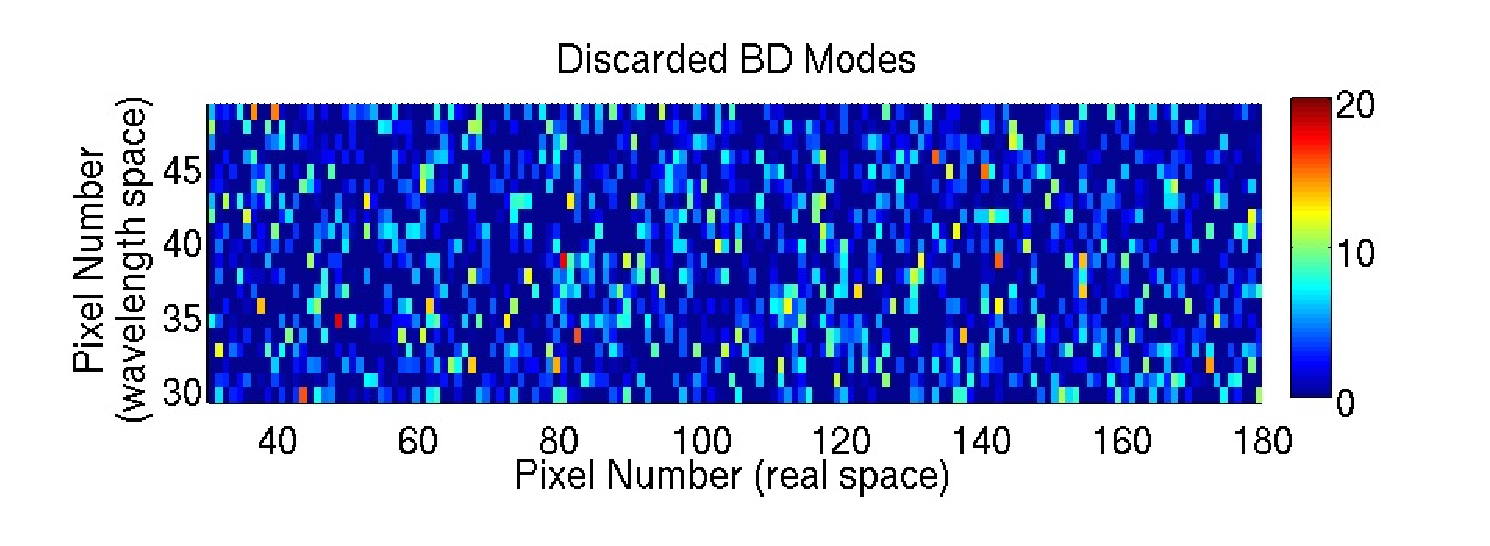
\includegraphics[width=4in]{BD_Discard}\caption{Noise reconstruction CCD frame, HIT-SI shot 129499, time 1.437 ms}\label{BD Noise}
\end{figure}
\end{center}


%%%%%%%%%%%%%%%%%%%%%%%%%%%%%%%%%%%%%%%%%%%%%%%%%%%%%%


\section{Fitting to the Data}\label{sec:Fit}
\subsection{Fit Function}
An elliptical gaussian function of the following form is fit to all channels at all timepoints:
\begin{equation}\label{Gaussian}
f(x,y,a)=\frac{V}{2{\pi}\sigma_x\sigma_y}exp\left(-\frac{1}{2}\left(\frac{(x-x_0)^2}{\sigma_x^2}+\frac{(y-y_0)}{\sigma_y^2}\right)\right)+f_0
\end{equation}
Where x and y are the spatial and wavelength directions, respectively, and `a' encapsulates the parameters: ${\sigma}_x$ is the spatial width, ${\sigma}_y$ is the wavelength width, $x_0$ and $y_0$ are the spatial and wavelength centers respectively, and $f_0$ is the background (continuum) offset level. It should be noted that in similar spectroscopic studies, fitting to a 1D gaussian is typical. For research using a PMT as the photon counter (such as \cite{cothran2006fast}), 1D fitting is a necessity, however, for studies using a CCD (\cite{den1994fast}\cite{rapisarda2007role}\cite{bamford1992combination}), where light could conceivably fall onto a 2D grid of pixels, gaussians are either binned in the spatial direction, or treated as if light falls only on a single column of pixels. If the fiber alignment is shifted slightly (ie: the spectrometer is bumped), an $x_0$ fixed to the calibration value will result in an artificially reduced $\sigma_y$, and therefore reduced temperature. We eliminate this source of error by allowing $x_0$ to vary as a free parameter. $X_0$ corrections of up to $\pm26\%$ of $\sigma_x$ are observed.\\
\subsection{Levenberg-Marquart Fitting}\label{sec::LM}
\hspace*{4ex}The model function $f(x,y,a)$ is fit to the data using the Levenberg-Marquardt Method (LMM). This is has been used in other plasma diagnostics to fit nonlinear or convolved models to data. Similar spectroscopic diagnostics\cite{Nikolić200167}\cite{Heesterman}\cite{Avdeeva} fit observed spectral gaussians using a convolved model of the continuum, the core ion profile, and the edge ion profile. Another work\cite{Pablant} uses the LMM to achieve tomographic inversion of the observed spectral profile, using an X-Ray diffraction spectrometer\cite{Reinke}. The LMM has also found use as a method to reconstruct 2D\cite{Luxon} or 3D\cite{Lazerson} MHD equilibrium profiles, by incorporating multiple diagnostic datasets.\\
\hspace*{4ex}The LMM, as derived independently by K. Levenberg\cite{LEVENBERG} and D. Marquardt\cite{marquardt1963algorithm}, combines the classical minimization techniques of linearizion (known alternately as the Taylor expansion method, or the Gauss-Newton method) and ``steepest descent'' (or, the gradient method). The former is used when the model has converged close to the solution, the latter when it is farther away. The LMM has been shown to have quadratic convergence\cite{Fan2005} under the relatively weak condition that $||F-f(x,y,a)||$, where F is the data, provides a local error bound. In contrast, Taylor expansion is invalid when the initial guess is far from optimal, as quadratic linearizion of the model is no longer a valid reconstruction, and gradient descent converges slowly when close to optimal, as the derivatives of the minimizing function ($||F-f(x,y,a)||$) are nearly zero (ie: Jacobian becomes rapidly singular (?????)), and the convergence tends to go as 1/tolerance (cite). The unweighted LMM algorithm is implemented as follows\cite{press1996numerical}\cite{nocedal2006numerical}:\\
\begin{equation}
\chi^2 = \frac{1}{2}||F-f(x,y,a)||^2
\end{equation}
Gauss-Newton Update:
\begin{equation}
\delta{a} = -[J^TJ(x_k)]^{-1}\nabla{\chi^2} = -[J^TJ(x_k)]^{-1}{J^T}(F-f(x,y,a))
\end{equation}
Gradient-Descent Update:
\begin{equation}
\delta{a} = \alpha\times\frac{\partial\chi^2}{\partial{a}} = \alpha\times{J^T}(F-f(x,y,a))
\end{equation}
The LMM combines the two, updating with the form:
\begin{equation}
(J^TJ+\lambda{I})\delta{P}=-J^T(F-f(x,y,a))
\end{equation}
The iteration proceeds with an initial $\lambda=.001$, and then increasing or decreasing by a factor of ten if the new value of $\chi^2$ is greater or smaller than the previous, respectively.

\hspace*{4ex}A further attractive property of the current implementation of the LMM is that it lends itself readily to the calculation of errors, not only of the overall model, but the standard parameter error as well. This ability to individually specify the errors in temperature and velocity represents a significant improvement over previous error propagation schemes in IDS instruments, which appear limited to RMS error, or S/N values. This is accomplished by approximating the covariance matrix of the final fit $f'$. Here, the hessian matrix $\mathcal{H}$ is approximated by $[J^TJ]$ (where $J$ has already been calculated), assuming small higher order residuals\cite{yuen2010bayesian}.
\begin{equation}
\sigma_P^2 =\mathrm{diag(covariance(f'))}= \mathrm{diag}(\sigma_{RMS}\mathcal{H}^{-1}) = \mathrm{diag}(\sigma_{RMS}[J^TJ]^{-1})
\end{equation}
Essentially, the rate of change of the model with respect to each parameter is scaled by the overall RMS error of the fit, producing standard parameter error. The above are all conveniently implemented in the \texttt{lm} Matlab package.

%%%%%%%%%%%%%%%%%%%%%%%%%%%%%%%%%%%%%%%%%%%%%%%%%%%%%%%%%%
\section{Calculation and Analysis}\label{sec::Analysis}
\subsection{Fitting to the Data}\label{sec::DataFit}
\hspace{4ex}An example of the velocity and temperature data returned by applying Eqn.\ref{Doppler_Eqns} to the gaussian fits is shown in figure \ref{Fig::Raw_VelTemp} for two visualization formats for HIT-SI and HIT-SI3.
\begin{figure}
\includegraphics[width=3in]{160728011L2Temp}\nolinebreak
\includegraphics[width=3in]{129499_Lines}\caption{Raw Temperature (L: HIT-SI3, C III, Toroidal Current and Injector Currents Given) and Velocity (R: HIT-SI, C III, Toroidal Current and Injector Phasing given for Shots 129499 (red) and 129496 (blue)), Two Visualization Schemes.}\label{Fig::Raw_VelTemp}
\end{figure}
Most experiments cited previously, including HIT-SI (\cite{Hossack_HitSi3}) have focused their analysis on the raw velocity and temperature data to extract flow and temperature profiles. This study improves upon this by isolating the component of the ion motion oscillating at the helicity injection frequency by fitting to a sinusoidal function. The initial parameter estimate is generated by a Fast Fourier Transform (FFT) of the data. Note that in contrast to BD, the dominant basis functions are expected to be periodic (if not sinusoidal), based on the periodic perturbation applied by the injectors. The data can be reconstructed, and additional information extracted, particularly the temporal phase and the average displacement. The functional form of the $i^{th}$ channel reconstructed velocity is:
\begin{equation}\label{Eqn::Fit_Fn}
v_i(t)=O_i+A_i\mathrm{Sin}(2{\pi}\:t\:f_{inj}+\phi)
\end{equation}
\begin{figure}
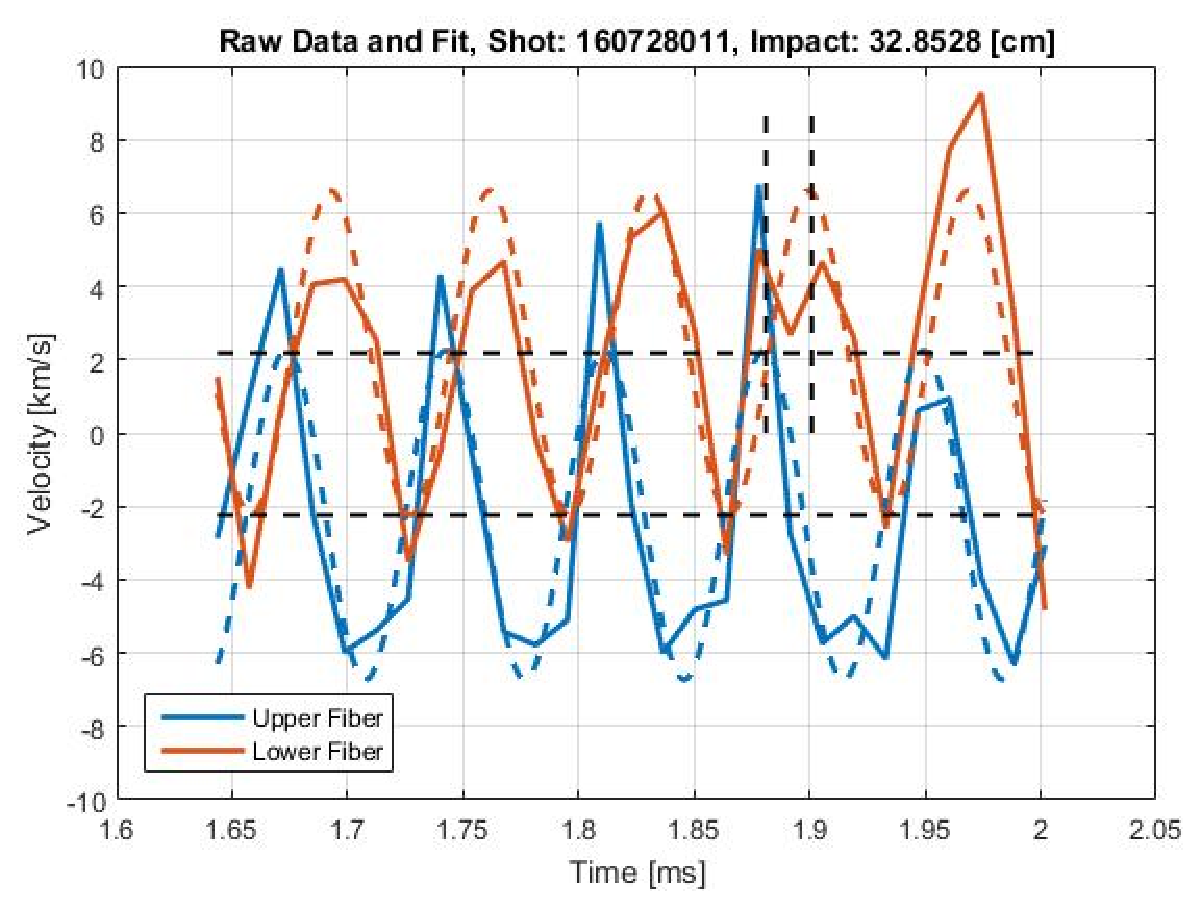
\includegraphics[width=4in]{ReconstExplain}\caption{HIT-SI3 raw velocity and fit. Shot and impact in figure. 
HIT-SI3 Velocity Reconstruction, and Visualization of Analyzed Quantities. Solid line: Raw Data, Dashed line: Functional Fit. Horizontal Black Line: Sine Fit Offset, Vertical Black Line: Phase Offset. Shot 160728011, Impact +32.8 cm (Blue) \& -32.8 cm (Orange) }\label{Fig::Reconst Explain}
\end{figure}
Where $O_i$ is the offset velocity, $A_i$ is the amplitude, and $\psi$ is the temporal phase offset. These quantities are illustrated in Fig.\ref{Fig::Reconst Explain}, which shows the sine-reconstruction of the velocity data for corresponding chords at impact parameter 32.8cm for HIT-SI3 shot 160728011. The differences in velocity offset, temporal phase, and amplitude are visible. While the injector frequency-correlated component (at 14.5kHz) of the signal in both temperature and velocity is obvious in Fig.\ref{Fig::Raw_VelTemp}, the validity of a single frequency fit is determined from the Fourier power spectrum of this component (and its higher harmonics) relative to all others, as shown in Fig.\ref{Fig::FFT Spect}.

\begin{figure}
\includegraphics[width=6in]{160728011L2L1VelSpect}\caption{Mode reconstruction: percentage of total FFT power spectrum contained at the injector frequency and its higher harmonics. HIT-SI3 shots XXXXXXX}\label{Fig::FFT Spect}
\end{figure}
\subsection{Calculated Quantities}\label{sec::CalcQuant}
From reconstructed data, the magnitude of the ion displacement can be calculated from the magnitude of the velocity oscillation, by analytic integration:
\begin{equation}
D_i=\frac{A_i}{{2\pi}\,f_{inj}}
\end{equation}
\hspace{4ex} offset velocity $O_i$ is related to the toroidal flow, but can also be affected by calibration errors in $y_0$ from Eqn.\ref{Gaussian}. On HIT-SI3, the dual-fiber views (Fig.\ref{HIT-SI3 Fibers Midplane}) allow the axisymmetric flow to be unambiguously calculated from the difference between velocity offsets of corresponding impact parameter above and below the geometric axis. HIT-SI did not have the lower viewport installed (Fig.\ref{HIT-SI Fibers Midplane}) and so the velocity after injector shutoff was used to define ``Zero Velocity''.\\
\hspace*{4ex}The temporal phase $\phi$ describes temporal relationship between ion motion and injector current. On HIT-SI, phase is referenced from the zero crossing of the ``x" injector (Fig XXX tank figure XXX). On HIT-SI3, it is referenced from that of the ``A" Injector (Fig XXX tank figure XXX). Phase correlations between channels show the extent of coherent structures in the plasma. In other words, regions of constant phase respond to the perturbation simultaneously.  In this analysis, three manipulations of the temporal phase are performed. First, the phase of all channels is decreased by $\pi/2$ to describe the displacement phase, instead of the velocity phase. Second, the phase of the upper fiber (the only array on HIT-SI) is lowered by $\pi$, so that the phase is now describing displacement in the positive toroidal direction rather than with respect to the detector. Finally, the phase for negative current shots is lowered by $\pi$ for all channels, so that the phase is now describing ion displacement in the toroidal current direction.   \\
\subsection{Error Analysis}\label{sec:ErrorAnal}
\hspace*{4ex}The errors associated with the flow, displacement, and temperature profiles can calculated directly (Eqn. \ref{Eqn::ErrCal}) from the parameter error output by the Levenberg-Marquardt algorithm (sec \ref{sec::LM}), and the RMS error associated with the sine-fit (Eqn.\ref{Eqn::Fit_Fn}).
\begin{equation}\label{Eqn::ErrCal}
\begin{split}
\sigma_{T_j} = \frac{\sqrt{\sum_i^T\sigma_{T_{i,j}}^2}}{T}\\
\sigma_{F_j}=\frac{\sqrt{\sum_i^T\sigma_{v_{i,j_u}}^2+\sigma_{v_{i,j_l}}^2}}{2*T}\\
\sigma_{D_j}=\frac{\sqrt{\sum_i^T\sigma_{v_{i,j}}^2+\sigma_{RMS}^2}}{T}\\
\end{split}
\end{equation}
Where T is the number of time points which the fit is performed over, $\sigma_{v_{i,j_{u,l}}}$ is the LM calculated error associated with velocity, for corresponding upper and lower impacts $j$ at timepoint $i$, $\sigma_{T_{i,j}}$ is the LM calculated error associated with temperature for chord $j$ and timepoint $i$, and $\sigma_{RMS}$ is the RMS error associated with the sine function fit.\\
\hspace*{4ex}The error associated with the temporal phase requires a more complecated calculation: RMS error is assumed to be locally gaussian in the phase-parameter space, and the width of this gaussian is proportional to the associated error. Specifically, we perturb the phase $\pm\pi$ of the fit, and compare the width of the curve of RMS error to the curve produced by the same operation applied to Eqn.\ref{Eqn::Fit_Fn} being fit to itself. Graphically, this is shown in Fig.\ref{Fig::Phase Error}. Note that the assumption of local gaussian error is clearly imperfect in the ideal error case.
\begin{figure}
\includegraphics[width=3in]{PhaseFitError}\caption{Calculation of Error Associated with Temporal Phase: Real and Ideal error describes changes in RMS error associated with perturbing Eqn \ref{Eqn::Fit_Fn} fit to the data and itself, respectively. Gaussian functions are fit to these curves.}\label{Fig::Phase Error}
\end{figure}

%%%%%%%%%%%%%%%%%%%%%%%%%%%%%%%%%%%%%

\section{Results}
\hspace{4ex}The results of these operations are plotted in Fig.\ref{Fig::PosNeg_HIT-SI3} and \ref{Fig::PosNeg_HIT_SI}, comparing ion species and toroidal current direction for both experiments. The C III and O II lines listed on the plots are the 464.7 and 464.9nm lines shown in fig.\ref{HITSI_CCD}. The O II line is weaker, resulting in noisier data. Ion toroidal displacement phase, flow velocity, maximum displacement, and temperature profile are calculated as in Sec \ref{sec::CalcQuant}, with error calculated as in Sec \ref{sec:ErrorAnal}. The HIT-SI3 lower fiber array (fig \ref{HIT-SI3 Fibers Midplane}) is plotted in Fig \ref{Fig::PosNeg_HIT-SI3} with dashed lines. The phases of the injectors are given alongside the phase of the displacement. The temporal phasing of the injectors is given as well.

\begin{figure}
\includegraphics[width=3in]{160525017L1Compare_extendedRange}\nolinebreak
\includegraphics[width=3in]{160525017L2Compare_extendedRange}\caption{HIT-SI3 0-120-240 injector phasing comparison of toroidal current direction. Toroidal displacement phase, toroidal flow, maximum displacement, and temperature profile given. Lower fiber array plotted with dashed line, upper array with solid line. Phase of injectors given, blue: injector a, orange: injector b, yellow: injector c. Shot number, toroidal current, gain in plot. Left: O II, Right: C III}\label{Fig::PosNeg_HIT-SI3}
\end{figure}
\begin{figure}
\includegraphics[width=3in]{129499_OII_ComparisonError_DataSuppression_2}\nolinebreak
\includegraphics[width=3in]{129499_CIII_ComparisonError_DataSuppression_2}\caption{HIT-SI 0-90 injector phasing comparison of toroidal current direction. Toroidal displacement phase, toroidal flow, maximum displacement, and temperature profile given. Injector phase given, blue: injector x, orange: injector y. Shot number, toroidal current, gain in plot. Left: O II, Right: C III}\label{Fig::PosNeg_HIT_SI}
\end{figure}

XXXX Note: Include alternate phasing/frequency for HitSi3/HitSi?XXXX



%%%%%%%%%%%%%%%%%%%%%%%%%%%%%%%%%%%%%%%%%%%%%%%%%%%%%%%%%%
\section{Discussion}
\hspace{4ex}A few general features of Fig  \ref{Fig::PosNeg_HIT_SI} and \ref{Fig::PosNeg_HIT-SI3} are worth mentioning. For temperature, the peaked profile in C III between 10 and 40 eV  is observed for both experiments. Furthermore, in HIT-SI3, the concurrence (XXXXXoverlap?XXX) of the upper and lower fiber arrays indicates an axisymmetric mean temperature profile, roughly 8eV hotter for positive toroidal current shots. The shape of the O II profile cannot be determined above error for HIT-SI or HIT-SI3, but is noticeably lower than C III for both. XXXX EXPLAIN THIS. Aaron says something about burnthrough time? XXX. \\
\hspace*{4ex}A strong peak at impact parameter of approximately 40 cm is observed in the ion displacement, of approximately 6 cm for C III and approximately 4 cm for O II in both experiments. This is roughly consistent with the expected outboard separatrix location (XXXXXX CITE XXXXX). The decrease in displacement magnitude may be due to the increased charge-to-mass ratio of C III vs O II.\\
\hspace*{4ex}The HIT-SI velocity profile cannot be unambiguously determined, outside of error, for C III or O II. For HIT-SI3, however, we find a small but statistically significant axisymmetric flow of $\approx3$km/s in negative current shots, decreasing towards zero for positive current shots.\\
\hspace*{4ex}The implications of the displacement phase are more complex. In HIT-SI, the relatively flat region observed for positive current and both ion species, between the two separatrices ($20\lesssim{R}\lesssim40$cm) implies that the spheromak is responding in a XXXXXX coherent XXXXXXX manner to the applied perturbation. The almost $180^o$ transition between the inboard separatrix and the geometric axis may imply XXXXX Something XXXXXX. These trends are not observed as clearly on the negative current shot. On HIT-SI3, a similar ``flat'' region is observed in the lower array, but not as much in the upper array. The inboard phase transition is not nearly as pronounced as in HIT-SI, and only appears in the upper array. On the outboard side, the two arrays show ion displacement locked to the closest injector (Fig. \ref{HIT-SI3 Fibers Midplane}). This implies that the observed displacement is either being pulled around by the motion of the injectors or is the perturbation itself. 

\section{Sources of Error}
\hspace*{4ex} \textbf{EVERYTHING}
\section{Conclusions}
\hspace{4ex}An Ion Doppler Spectrometer diagnostic system has been constructed which fulfills the requirements of spatiotemporal resolution, and spatial extent, on the HIT-SI and HIT-SI3 devices. Sub-injector timescale framerates (up to $8\times{14,500}$Hz and complete mid-plane reconstruction (on HIT-SI3) with up to 72 spatial channels have been produced, for C III and O II. Careful calibration and filtering and fitting algorithms allow errors to be specified at $\lesssim1$ km/s and $\lesssim5$ eV, with an instrument temperature of 8-16 eV for C III. Fitting to the data has found axisymmetric temperature profiles on HIT-SI3 for C III in agreement with the upper midplane on HIT-SI, peaked near the inboard separatrix at $\approx40$eV. Axisymmetric displacement profiles have been found on HIT-SI3, peaked at the outboard separatrix with a magnitude $\approx8$ cm, in agreement with the upper midplane on HIT-SI. Axisymmetric, current dependent flow profiles have been found on HIT-SI3, up to 3 km/s. Finally, coherent toroidal ion displacement, locked to the applied perturbation, is seen in both experiments. Further work will investigation the differing results between ion species, potentially with atomic modeling. Both the acquisition and analysis capabilities of the system here described are higher than that of other IDS systems described in literature. It is hoped that replication of this system, in whole or part, will be beneficial to future researchers.


\section{Acknowledgments}
The Authors would like to acknowledge the assistance of the rest of the HIT-SI team: Kyle Morgan, Derek Sutherland, Chris Everson, James Penna, Professor Brian Nelson, and John Rogers.


Possible Topics for discussion:
\begin{enumerate}
\item Positive vs Negative current (Check)
\item Comparison of Temperature Evolution to Model
\item Velocity oscillations/Separatrix position calculation (kinda Check)
\item Comparison to Simulation (In forthcomming paper)
\item Different Frequency/Phasing (Incomparable? no HF HITSI3 data?)
\item OII vs CIII (we have the ability to do this)
\item Radial Shift Due to Flow
\item Beta

\item Analysis from the raw data (without FFT)
\item Analysis with FFT (contained in previous paper)
\end{enumerate}


%%%%%%%%%%%%%%%%%%%%%%%%%%%%%%%%%%%%%%%%%%%%%%%%
\newpage
\section{References}



\bibliographystyle{unsrt}
\bibliography{Bibleography}
\begin{comment}
\begin{thebibliography}{}
% Fitting to Data References
\bibitem{1} \begin{verbatim}http://www.sciencedirect.com/science/article/pii/S0022407300001230}\end{verbatim}
\bibitem{2}\begin{verbatim}http://iopscience.iop.org/article/10.1088/0029-5515/22/6/009/meta\end{verbatim}
\bibitem{3}\begin{verbatim}http://iopscience.iop.org/article/10.1088/0029-5515/55/2/023009/meta\end{verbatim}
\bibitem{4}\begin{verbatim}http://iopscience.iop.org/article/10.1088/0741-3335/54/10/105022/meta\end{verbatim}
\bibitem{5}\begin{verbatim}http://www.euro-fusionscipub.org/wp-content/uploads/2014/11/EFDC020302.pdf\end{verbatim}
\bibitem{6}\begin{verbatim}http://aip.scitation.org/doi/full/10.1063/1.4891977\end{verbatim}
\bibitem{7}\begin{verbatim}http://aip.scitation.org/doi/10.1063/1.4758281\end{verbatim}
\bibitem{8}\begin{verbatim}http://iopscience.iop.org/article/10.1088/1742-6596/666/1/012002/pdf\end{verbatim}
\bibitem{9}\begin{verbatim}http://epubs.siam.org/doi/pdf/10.1137/0111030\end{verbatim}
\bibitem{10}\begin{verbatim}http://www.jstor.org/stable/43633451?seq=1#page_scan_tab_contents\end{verbatim}
\bibitem{11}\begin{verbatim}http://link.springer.com/article/10.1007/s00607-004-0083-1\end{verbatim}
\bibitem{12}Bamford, 1992
\bibitem{13}Hartog 1994
\bibitem{14}Rapisarda, 2007
\bibitem{15}\begin{verbatim}http://www.apmath.spbu.ru/cnsa/pdf/monograf/Numerical_Optimization2006.pdf\end{verbatim}
\bibitem{16}Numerical recipies in C
\bibitem{17}\begin{verbatim}http://onlinelibrary.wiley.com/doi/10.1002/9780470824566.app1/pdf\end{verbatim}

% Experimental Setup
\bibitem{18}AARONS THESIS

% BD filtering
\bibitem{19}\begin{verbatim}http://aip.scitation.org/doi/pdf/10.1063/1.1321739\end{verbatim}
\bibitem{20}\begin{verbatim}http://aip.scitation.org/doi/pdf/10.1063/1.870481\end{verbatim}
\bibitem{21}\begin{verbatim}http://aip.scitation.org/doi/pdf/10.1063/1.872796\end{verbatim}
\end{thebibliography}}

\end{comment}

\end{document}
